\documentclass[11pt]{letter}
\usepackage[a4paper,left=2.5cm, right=2.5cm, top=2.5cm, bottom=2.5cm]{geometry}
\usepackage{color}
\usepackage[usenames,dvipsnames]{xcolor}
\usepackage[colorlinks = true, urlcolor = blue]{hyperref} %hyperlinks
\usepackage[osf]{mathpazo}
\usepackage{graphicx}
\usepackage{amsmath,amssymb}
\signature{Thomas Guillerme \\ Natalie Cooper}
\address{Zoology building \\ Trinity College Dublin \\ Dublin 2, Ireland \\ \\ guillert@tcd.ie}
\longindentation=0pt
\begin{document}

\begin{letter}{}

\opening{Dear Dr Fontaneto,}

RE: PLOS ONE Decision: PONE-D-15-05911 - [EMID:ffa50492e76c2059]

Please find enclosed our resubmission of our manuscript ``Effects of missing data on topological inference using a Total Evidence approach". We include below details of how we have dealt with the reviewer's comments. Your comments and the reviewer's comments are in blue and our responses are in black.

We would however, first like to draw your attention to a couple of points. Firstly, while we understand the difficulties of obtaining reviewers for papers, we were very disappointed to have the previous decision made based on just one review. Secondly, we would like to clarify that we did use statistics (see our response to comment A below), we just used statistics that do not produce p-values. We therefore feel that the reviewer has slightly misunderstood the statistics we applied in the manuscript and respond to this in detail below.

\textcolor{blue}{
Dear Mr Guillerme, \\
Thank you for submitting your manuscript to PLOS ONE. After careful consideration, we have decided that your manuscript does not meet our criteria for publication and must therefore be rejected. \\
First of all, apologies for the long delays. We immediately received the comments from the first reviewer and in the meanwhile another reviewer agreed to send us comments but failed to do so, even after several reminders. Thus, I now have to reach a decision with only one reviewer.
Unfortunately, the comments from the only reviewer we have are rather negative and the problems that have been highlighted too many. Please, go through all the comments of the reviewer: I think that they all make sense and should be addressed and solved to produce a more convincing and less ambiguous story. \\
If you think that the issues can be solved by new analyses, we will be happy to reconsider a new version of the manuscript as a re-submission. \\
I am sorry that we cannot be more positive on this occasion, but hope that you appreciate the reasons for this decision. \\
Yours sincerely, \\ \\
Diego Fontaneto \\ 
Academic Editor \\
PLOS ONE}

\textcolor{blue}{Reviewers' comments:}

\textcolor{blue}{1. Is the manuscript technically sound, and do the data support the conclusions?}

\textcolor{blue}{Reviewer $\#$ 1: No}

See our detailed response below.

\textcolor{blue}{2. Has the statistical analysis been performed appropriately and rigorously?}

\textcolor{blue}{Reviewer $\#$ 1: No}

See our detailed response below.

\textcolor{blue}{3. Does the manuscript adhere to the PLOS Data Policy?}

\textcolor{blue}{Reviewer $\#$ 1: No}

We apologise for the confusion here. We mentioned where our data was stored in the supporting information but forgot to add this under the ``Data Reproducibility and Availability" section in the manuscript. We have now corrected this. All the data generated by the simulations are directly available on \href{http://figshare.com/articles/Effect_of_missing_data_on_topological_inference_using_a_total_evidence_approach/1306861}{FigShare} (goo.gl/h5Kxb5). Note that along with the data we share the full code used for repeating the submitted manuscript, from simulating the data to generating the figures and compiling the manuscript available on \href{https://github.com/TGuillerme/Total_Evidence_Method-Missing_data}{GitHub} (goo.gl/ewRsrm). All this code is provided with a detailed description of each step that we are happy to develop if needed.

\textcolor{blue}{4. Is the manuscript presented in an intelligible fashion and written in standard English?}

\textcolor{blue}{Reviewer $\#$ 1: Yes}

\textcolor{blue}{5. Review Comments to the Author}

\textcolor{blue}{Reviewer $\#$ 1: This paper tackles an interesting questions. Despite some problems noted below, the experimental design seems adequate.}

%-------------

\textcolor{blue}{A - Unfortunately the data analysis performed is simply the calculation of a number of summary statistics about the overlap between the estimates returned for different simulation conditions. I suspect that if the authors take some time to do statistics (calculate some P-values, confidence intervals, or take a Bayesian perspective), they'll be able to make a statistical case for most of the points that they are trying to make. But I just don't think that a simulation comparison should be publishable without *some* statistical analysis (beyond the calculation of summaries).}

We feel that the reviewer has slightly misunderstood the statistics we applied in this manuscript. The purpose of ANOVAs or multiple regression (see suggestion from comment 20 below) is to compare differences in means across groups and test whether they are different from what one would expect according to a null model. In contrast, in our simulation approach, we essentially have access to a representative sample of the entire population distribution of tree topology comparisons. Therefore, we can simply ask whether these distributions are different when our missing data parameters varies by comparing them directly. One standard such approach to comparing distributions directly is to use the Bhattacharyya Coefficient. This number has direct interpretation in a probablistic sense and is simply the probability that the two distributions are the same. If the two distributions overlap completely then they have Bhattacharyya Coefficient and probability of being the same of 1. At the other extreme, if the two distributions are completely disjointed, then they have a Bhattacharyya Coefficient and hence probability of being the same of 0 (line 306 and 307 in the previously submitted manuscript and lines 320 and 319 in our revision). Thus, the Bhattacharyya Coefficient is a probability, comparable to, but not the same as, a p-value that could be calculated using frequentist approaches such as t-tests, ANOVAs or GLMs.

Furthermore, as a direct comparison of two known distributions, using the the Bhattacharyya Coefficient comes with far fewer statistical assumptions than are required in ANOVAs, GLMs and their analogues. For example, the direct comparison approach using Bhattacharyya Coefficient is capable of comparing a multi-modal distributions whereas the assumption of normality required in a ANOVAs or GLMs thus using them would inviolate the robustness of the resultant p-value. There is an additional complication to using ANOVAs or GLMs in simulation type analyses arising from having access to very large sample sizes (e.g. 50000 data points for the Maximum Likelihood bootstraps trees and the Bayesian posterior distribution trees) that leads to p-values shrinking to zero and resulting in comparisons being almost certain to yield ``statistically significant" differences in the mean (see the figure below; code for reproducing it is available from \href{https://github.com/TGuillerme/Total_Evidence_Method-Missing_data/blob/master/Analysis/Comparing_distribution_example.R}{https://goo.gl/4djNUf}). We argue that in this situation, it is better to compare the entire distribution using the Bhattacharyya Coefficient rather than simply the means. Additionally, because we are comparing topologies in this manuscript, we made the methodological choice to use the modal topology (i.e. the most represented topology) instead of the mean topology (i.e. a hypothetical ``middle'' topology).

Finally, we would like to underline that we report our 50\% and 95\% confidence intervals in Figures 4 and 5 when showing the effect of the missing data parameters (calculation detailed lines 295-295) as well as the 1st and 3rd quartiles when comparing the methods in Table 1.

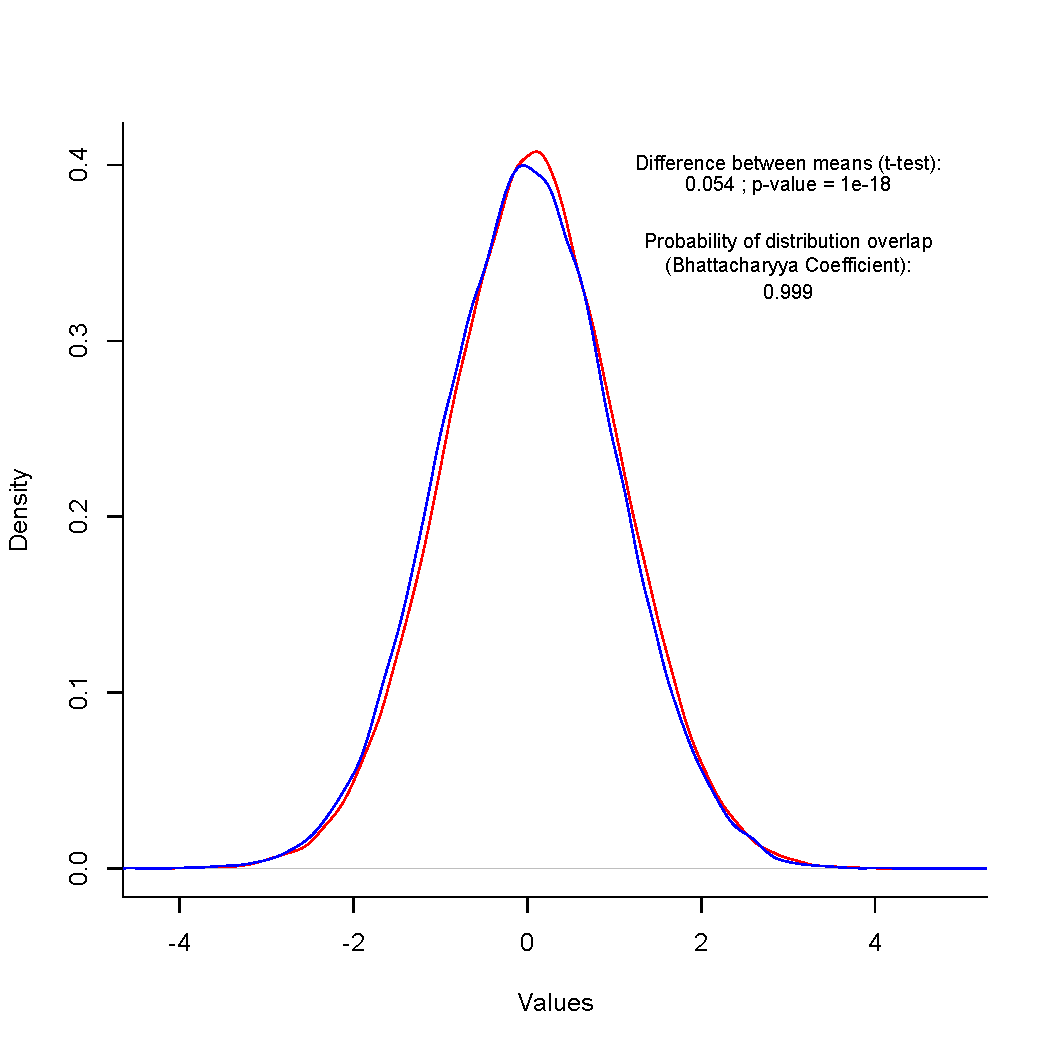
\includegraphics[scale=0.8, keepaspectratio=true]{Comparing_distributions.pdf} \\
\textit{The figure shows two extremely similar distributions. However, although the Bhattacharyya Coefficient shows that the distributions are really similar (0.999 overlap probability), a frequentist approach (simple t-test) suggests that there is a significant difference between the means (p-value $<$ 0.0000001). This highlights the reason we chose to use the Bhattacharyya Coefficient in our manuscript.}

%-------------

\textcolor{blue}{B - The bias in the analysis in favor of Bayesian methods makes the recommendation to use Bayesian methods less satisfying.}

The reviewer is (we believe) referring to comment 13 below. We would like to emphasize that in this study we focused on the effect of missing data in the morphological part of the matrix on topology only, and we are ignoring branch lengths. The choice of the following priors (``exponential prior on the shape of the gamma distribution of $\alpha$ = 0.5 for both partitions" (line 228 in the previously submitted manuscript and line 240 in our revision) and the ``transition/transversion ratio prior of two sampled from a strong beta 229 distribution ($\beta$(80,40))" (line 229 in the previously submitted manuscript and line 241 in our revision)) affected mainly the molecular part of the matrix that remains constant (gamma distribution and transition/transversion ratio) and were a minor part of the MCMC sampler (2.17\% of the moves of the MCMC sampler for the three priors combined). Therefore we are confident that the topology is minimally affected by the priors, allowing us to explore the effect of missing morphological data on topology as well as reducing our computational time to a realistic 1.4 CPU centuries. Note that the use of the ``the ``true" tree's topology'' (line 226 in the previously submitted manuscript and line 237 in our revision) as a starting tree is not a prior and was used to avoid the chains getting stuck in local optima.

We clarified these points in the manuscript as follows:

Lines 248 to 249 in our revision:

\hfill\begin{minipage}{\dimexpr\textwidth-1cm}
Each Bayesian tree was estimated using two runs of four chains each for a maximum of 5$\times$$10^7$ generations. For each estimation, we used the ``true" tree's topology as a starting tree (with a starting value for each branch length of one). We also used two priors on the molecular part of the matrix: an exponential prior on the shape of the gamma distribution of $\alpha$ = 0.5, and a transition/transversion ratio prior of two sampled from a strong beta distribution ($\beta$(80,40)); and one prior on the morphological part of the matrix (exponential prior on the shape of the gamma distribution of $\alpha$ = 0.5). We used these priors to speed up the Bayesian estimation process. These priors biased the way the Bayesian process calculated branch lengths by giving non-random starting points and boundaries for parameter estimation however, here we are focusing on the effect of missing data on tree topology and not branch lengths. Even using these priors, it took $~$ 140 CPU years to build 50 sets of 125 Bayesian trees (2.30GHz clock speed nodes). The detailed MrBayes parameters are available in the Supporting Information S1.
\end{minipage}

\textcolor{blue}{C - The use of Mk rather than Mkv makes the study less relevant to real data analyses.}

Throughout our manuscript, we referred the M\textit{k} model \textit{sensu} Lewis 2001 (a Q-matrix with \textit{k} character states and an equal substitution rate $\mu$). The M\textit{kv} model is identical to the M\textit{k} model (as described in Lewis 2001) however, in practice, it assumes that all characters are variable and that therefore, one should correct for acquisition bias that can induce branch length inflation. This is generally done by using an algorithm in the phylogenetic software that adds ``dummy'' morphological characters. In some software (e.g. GARLI or BEAST), it is important to specify whether the morphological data should be corrected for acquisition bias or not (M\textit{k} or M\textit{kv} options). However, in RAxML and MrBayes, this bias is corrected automatically by addition of ``dummy'' characters and M\textit{k} just designates the evolutionary model used with $\mu$ $\geq$ 0 (e.g. Nylander \textit{et al.} 2004 - Systematic Biology). 

The reviewer is of course correct in that real data rarely contain invariable morphological characters, because these don't contribute to phylogenetic signal. Our simulated data, on the other hand, will occasionally contain invariable characters merely because of missing data, therefore we made the decision to describe the model for morphological character evolution as the M\textit{k} evolutionary model ($\mu$ $\geq$ 0 rather than the M\textit{kv} model where $\mu$ $>$ 0). RAxML and MrBayes do however correct for acquisition bias as implemented in their algorithm for dealing with morphological data.

However, following the reviewer's comment, we changed the designation of the model from M\textit{k} to M\textit{kv} in the text, to underline that we corrected for acquisition bias. We also explicitly mentioned it in the revision in the following lines:

Lines 208 to 209 in our revision:

\hfill\begin{minipage}{\dimexpr\textwidth-1cm}
We used RAxML because it automatically corrects for acquisition bias (Lewis 2001). It is also heavily used in the literature for Maximum Likelihood tree inference (e.g. [...]) and is one of the fastest methods available (Stamatakis 2008).
\end{minipage}

Lines 233 to 234 in our revision:

\hfill\begin{minipage}{\dimexpr\textwidth-1cm}
Note that MrBayes automatically corrects for acquisition bias in the morphological data partition (Nylander \textit{et al.} 2004; Ronquist \textit{et al.} 2012).
\end{minipage}

%-------------

\textcolor{blue}{D - Many of the equations are incorrect.}

We thank the reviewer for pointing out the two errors in the equations in the main body of the text at lines 258 and 275 (see our detailed response to comments 15 and 17 below). Also we recognise that the equations in our ``Supporting Information S2: Tree Comparisons'' are confusing and are actually unnecessary for the understanding of this manuscript. We therefore removed the details of the Robinson-Foulds and Triplets distances from the ``Supporting Information S2: Tree Comparisons'' section.

%-------------

\textcolor{blue}{E - If there was a mention of the data being deposited, I missed it. I apologize if I did miss it.}

We apologise again for the confusion here. See our comment above on ``Data Availability and Reproducibility".

%-------------

\textcolor{blue}{-------------------------}

\textcolor{blue}{Some specific concerns:}

\textcolor{blue}{1 - line 25 and elsewhere: incorrect smart quotes in ``best", ``classical"...}

We fixed the smart quotes in our revision.

%-------------

\textcolor{blue}{2 - line 88 ``used it to infer a matrix" $->$ ``used it to simulate a matrix". ``inference" is used in place of simulation elsewhere.}

We changed ``infer" to ``simulate" both at line 88 and in the Figure 1 caption.

%-------------

\textcolor{blue}{3 - line 112: does diversitree just stop simulating when it reaches the correct number of tips, or does it deal with the biases that can result from doing that? (Stadler 2011 is the ref for a discussion of this issues, I believe)}

See our response to comment 6 below.

%-------------

\textcolor{blue}{4 - line 113: ``rates from a uniform distribution" with what upper and lower bounds?}

Both birth ($\lambda$) and death ($\mu$) parameters are probabilities bounded between 0 and 1. We have added this to the new version of the manuscript.

%-------------

\textcolor{blue}{5 - line 118: with 25 living and 25 fossil taxa. Are the fossils just put at the extinction point for the extinct lineages?}

Yes. We have clarified as follows in our revision (lines 118 to 119):

\hfill\begin{minipage}{\dimexpr\textwidth-1cm}
[We] select only trees with 25 living and 25 fossil taxa. The fossil taxa were considered as unique tips at the end of extinct lineages.
\end{minipage}

%-------------

\textcolor{blue}{6 - line 110 - line 120. The procedure for generating a tree with fossils is a valid procedure. But it is idiosyncratic, which will make these results harder to relate to other work. Easy of comparability with other work is one of the advantages of using formally characterized models. In this case, I think that using the TreeSim package would have led to a study with higher impact. This part of the methods section would be reduced to stating the parameter values chosen, and other workers could study similar tree generation simulations. As it stands, it is unlikely that other workers will every generate trees in precisely the way that the authors do. Thus, there will always be a ``however, Guillerme and Cooper generated their trees under a different model..." caveat necessary when discussing this work in the context of other work.}

We do not agree that the procedure is idiosyncratic. \texttt{diversitree} and \texttt{TreeSim} both generate birth-death trees in the same way (although \texttt{diversitree} is slightly quicker) and are well curated and maintained. We chose to use the \texttt{diversitree} package because we are more familiar with it. We could also have used a number of other packages including \texttt{TESS}. We are also by no means the only people using the \texttt{diversitree} package - the paper associated with it (FitzJohn 2012, Methods in Ecology and Evolution) has been cited three times more (155 cites on Google Scholar) than the publication associated with the \texttt{TreeSim} package (Stadler 2011, Systematic Biology - 55 cites on Google Scholar).

We also disagree that using \texttt{TreeSim} would reduce the amount of explanation required. We believe that carefully outlining our methods will help people repeat our analyses. Thus we would describe any \texttt{TreeSim} analysis in just as much detail.
Finally of course no one can repeat our analyses precisely as we used random parameters to avoid biasing the analyses towards a particular type of tree. However, we do provide all these trees in the supporting information (``Data Reproducibility and Availability" section; \href{http://figshare.com/articles/Effect_of_missing_data_on_topological_inference_using_a_total_evidence_approach/1306861}{FigShare} link (goo.gl/h5Kxb5)) so future workers can fully repeat our analyses. Thus we feel that repeating the entire set of simulations (1.5 CPU centuries worth) using \texttt{TreeSim} is not necessary and would not influence our results or their utility to future workers.

%-------------

\textcolor{blue}{7 - line 126 ``random base frequencies" is too vague. Dirichlet(1, 1, 1, 1) perhaps?}

We have clarified as follows:

Lines 126 to 129 in our revision:

\hfill\begin{minipage}{\dimexpr\textwidth-1cm}
The matrix [...] was generated [...] using the HKY model with random base frequencies (sampled from a uniform probability distribution bounded between 0 and 1 with the total frequency for the four bases equal to 1)[...]
\end{minipage}

%-------------

\textcolor{blue}{8 - Do the simulations apply ascertainment biases as described by Lewis' Mkv (2001) model? It seems like they should... At minimum, the point should be discussed.}

See our response to comment C above.

%-------------

\textcolor{blue}{9 - line 171 - 177: the authors need to explain the order of operations for the $M_F$ vs $M_C$ masking. It makes a difference. If you mask out $M_F$ percentage of cells, and then mask $M_C$ percentage of columns, it is possible (indeed very probable) that the percentage of missing data in fossil characters that remain will not be $M_F$ after some of the morphological columns are removed. If you mask by $M_C$ first, and then $M_F$, the resulting matrices will always have $M_F$ percentage missing data (modulo rounding error) in the simulated realizations.}

We clarified this point ($M_C$ comes second) in the new version of the manuscript (lines 173 to 183). We also clarified the potential confusion between the amount of data removed in one parameter ($M_F$ = 10\% for example) and the amount of missing data in the morphological matrix (5\%) in the same revised paragraph (lines 173 to 183).

\hfill\begin{minipage}{\dimexpr\textwidth-1cm}
In practice, each parameter represents a different way of removing data from the matrix: $M_L$ removes rows from the living taxa's data; $M_F$ removes cells from the fossil taxa's data; and $M_C$ removes columns across both living and fossil taxa's data. Note that $M_L$ and $M_F$ differ not only because of the region of the matrix affected: for $M_L$ all the morphological data of a percentage of living taxa are removed, whereas for $M_F$ a percentage of the data are removed at random from across the whole of the morphological matrix for fossil taxa. We first applied the parameters $M_L$ and $M_F$ to the matrix and then applied the $M_C$ parameter. Therefore, when 10\% data was missing for both $M_L$ and $M_F$, 10\% data was missing in the morphological part of the matrix. However, when applying the $M_C$ parameter with the same percentage (10\%) the resulting matrix potentially had more than 10\% data missing.
\end{minipage}

%-------------

\textcolor{blue}{10 - Header for 3. should be ``building phylogenetic estimates" or ``estimating phylogenies" because the previous section described how the phylogenies and character data were ``built."}

We changed the Header 3 to ``Estimating phylogenies".

%-------------

\textcolor{blue}{11 - RAxML searching: it would be nice to see some searches started from the true tree. This is clearly not an option for real data sets, but it is helpful in simulation studies because it lets the reader determine if the results could be an artifact of insufficient tree searching.}

Our simulations were designed to test the effects of missing data in as realistic a manner as possible given computational constraints. Thus, we do not feel that this additional analysis would add much to the manuscript, especially since it is already rather long and complex. 

%-------------

\textcolor{blue}{12 - Filtering the data sets for strong bootstrap support under the full data analysis surely introduces some bias in favor of the no-missing data analyses.}

We implemented this step of keeping trees with a minimum total median bootstrap to make the topological comparisons more robust. If the no-missing data tree has low node support, it is likely that the changes in topology for the missing data trees are not linked to our focal question (the effect of removing characters, living taxa or fossils) but just to the low supported nodes. In fact, because we repeat the tree inference 125 times ($5^3$ parameters combinations), it is likely that we have 125 different pseudo-random solution for the nodes with really low phylogenetic support and that, therefore, the observed changes in topologies are just linked to the pseudo-random replication. Note however that we did not exclude this scenario from our protocol; the trees selected with a median bootstrap $>$ 50 could well contain some unresolved nodes with a low bootstrap ($<$ 50). We've added the following justification in our revision (lines 215 to 220):

\hfill\begin{minipage}{\dimexpr\textwidth-1cm}
We repeated this selection until we obtained 50 sets of simulations (i.e. 50 ``complete" and 50 x 125 ``missing-data" matrices) with a relatively strong phylogenetic signal (median bootstrap $>$ 50). This step was implemented to make sure that the differences we observed in topologies (see below) were due to the amount of missing data for each parameter ($M_L$, $M_F$ and $M_C$) and not simply to low branch support that is likely to lead to different topologies.
\end{minipage}

%-------------

\textcolor{blue}{13 - MrBayes: using strongly informative priors for the true parameters does more than speed up the searching, it represents an ``unfair" advantage (an option that would not be available in real data analysis in which one does not know the true values) for the Bayesian method. This makes the studies report of superior behavior of Bayesian methods less persuasive.}

See our response to comment B above.

%-------------

\textcolor{blue}{14 - line 254: RF measures the difference between the number of clades and the twice number of shared clades across two trees. The statement that it ``measures the number of shared clades across two trees" should be revised.}

We revised this statement lines 267 to 269 in our revision:

\hfill\begin{minipage}{\dimexpr\textwidth-1cm}
The Robinson-Foulds distance, or ``path difference", measures the difference between the number of clades and the twice number of shared clades across two trees.
\end{minipage}

%-------------

\textcolor{blue}{15 - line 258: RF is 0 (not 1) when the trees are identical. It's maximum (for 2 rooted binary trees) is 2(n-2) not n-2.}

We thanks the reviewer for pointing out this error and we changed the following sentence (lines 271 to 273 in our revision):

\hfill\begin{minipage}{\dimexpr\textwidth-1cm}
This metric is bounded between zero, when the two trees are identical, and $2(n-2)$ (for two trees with $n$ taxa) when there is no shared clade in the two trees.
\end{minipage}

%-------------

\textcolor{blue}{16 - The ``scaling" to produce the Normalized RF ``distance" is confusing. It is also inverting the sign of the distance, so it has become a measure of similarity.}

We agree that this is confusing and thank the reviewer for pointing this out. We changed the mentions of ``Normalised Robinson-Foulds distance'' and ``Normalised Triplets distance'' to ``Normalised Robinson-Foulds metric'' and ``Normalised Triplets metric'' throughout the our revision. Additionally, we clarified the scaling method as follows (lines 276 to 284 in our revision):

\hfill\begin{minipage}{\dimexpr\textwidth-1cm}
We normalised this metric following Bogdanowicz \textit{et al.} (2012)'s Normalised Tree Similarity (NTS) method. This methods scales any tree comparison metric using the mean distance between 1000 random trees (see Supporting Information S2: Tree Comparisons for the calculation details). This method is a generalisation of the topological accuracy method (Price \textit{et al.} 2010) allowing to compare topological differences between any tree with any tree comparison metric. In practice when the Normalised Robinson-Foulds metric between two trees is equal to one, the trees are identical; if the metric is equal to zero, the trees are no more different than expected by chance; finally if the metric is less than zero, the trees are more different than expected by chance. Note that once rescaled, the Normalised Robinson-Foulds metric is a measure of similarity, rather than of distance like the original Robinson-Foulds metric. 
\end{minipage}
%-------------

\textcolor{blue}{17 - line 275: why isn't the upper bound of the triples distance n choose 3 (instead of n choose 4). I think you got the formula from an unrooted quartet distance.}

We corrected this error lines 290 to 291 in our revision:

\hfill\begin{minipage}{\dimexpr\textwidth-1cm}
It is bounded between zero when the two trees are identical and $\binom{n}{3}$ (for two trees with $n$ taxa) when there is no shared taxa/clade position in the two trees.
\end{minipage}

%-------------

\textcolor{blue}{18 - Using the BC stat may be similar in spirit to using a t-test, but it is not equivalent.}

We clarified this point in the text as well as in the figures 2 and 3 captions (``equivalent" $->$ ``comparable" ; lines 324 to 326 in our revision):

\hfill\begin{minipage}{\dimexpr\textwidth-1cm}
Note that this is comparable to performing a two-sided t-test, but we use the Bhattacharyya Coefficient here because we are comparing whole distributions not just their means.
\end{minipage}

%-------------

\textcolor{blue}{19 - Figure 3: B is confusing. If both curves are probability distributions, then they both have to integrate to 1. So B(y) can't cover just a subset of the area covered by B(x).}

We thank the reviewer for pointing out this error. We fixed the shape of the distribution in Figure 3B.

%-------------

\textcolor{blue}{20 - ``Combined effect of missing data parameters" section ANOVA or multiple regression are the appropriate analyses to tease apart multiple interacting factors. Here the authors opt to describe results without statistical tests, which is disappointing.}

See our detailed response to comment A above.

%-------------

\textcolor{blue}{21 - line 398: ``mMthods" $->$ ``Methods"}

We thanks the reviewer for pointing out this typo and fixed it.

\textcolor{blue}{22 - line 420: contra the statement here, a consensus collapsing to a polytomy will affect the RF distance (could go up or down, but it will change).}

We revised this statement at lines 436 to 444 in our revision:

\hfill\begin{minipage}{\dimexpr\textwidth-1cm}
In this case, the Normalised Robinson-Foulds metric will decrease when the fossil is present at a lower taxonomic level (i.e. separated with more nodes from the root) but affects the clade conservation less at higher taxonomic level (i.e. separated with less nodes from the root). Conversely, because a fossil in a high taxonomic level clade has many chances to branch on different nodes within the clade, it will be more likely to act as a wildcard taxa and decrease the Normalised Triplets metric. Therefore, the $M_{F}$ parameter is likely to affect the Normalised Robinson-Foulds metric less than the Normalised Triplets metric for the Bayesian consensus trees.
\end{minipage}

%-------------
\textcolor{blue}{Supplement 2:}

\textcolor{blue}{23 - more confusion about the min RF here. Also note that if you are counting the entire leaf set as a clade (e.g the star tree having N=1), then the number of clades in rooted binary tree is n-1 (not n-2). Equation 3 has an extra ``-2" As stated it implies that the max RF distance for n=3 is 0, when the correct answer is 2.}

See our response to comment D above.
%-------------

\textcolor{blue}{24 - The definition of the scaled RF implies that it is never positive (sinc the numerator cannot be positive and the denominator is positive).}

See our response to comment D above.
%-------------

\textcolor{blue}{25 - The decision to use Yule trees as the base line for the mean distance is not explained, and seems odd given that the true tree are not Yule trees. I'm not sure that it makes much difference, but it is odd.}

We followed the protocol in the cited reference (Bogdanowicz 2012) where the normalisation of the metrics is done on the mean value of that metric when compared to random trees. Using random Yule trees is the best way to generate purely random trees since they are not based on any evolutionary model and take only one parameter, the number of tips, as opposed to the Birth-Death tree that use a more realistic evolutionary model and take multiple parameters.
%-------------

\textcolor{blue}{26 - The NTS can only -infinity for distances that have the property that the mean distance between random Yule trees is 0. This is not true of either distance metric here. So the real range of values is (mean-max)/mean for both the RF and triples distance.}

As clarified in our revision (lines @276 to @284), the NTS is a generalisation of the topological accuracy method (Price \textit{et al.} 2010 PLoS ONE) and is therefore not specialised for the RF or the Triples distance.
%-------------

\textcolor{blue}{27 - Note that JavaScript is a language, so it a bit confusing to refer to a Java program as a ``Java script."}

We fixed this typo.
%-------------

\textcolor{blue}{28 - Equation (6) is not correct. You shouldn't set the summation sign as the left hand side of an equation because the notation has a standard definition. More importantly, the $\#$ of triples is the number of ways of drawing 3 (unordered) leaves from the leaf set. So it is n choose 3 not n choose 4.}

See our response to the comment D above.
%-------------

\textcolor{blue}{29 - Equation (7) is true for a three-leaf tree with a polytomy occurring with probability = 1/4 and the other 3 trees being equiprobable. I don't think that is is true for any other weighting of trees for other numbers of taxa. It might be, but the authors must show this.}

See our response to comment D above.
%-------------

\textcolor{blue}{30 - I don't think that equations 8, 9, or 10 are correct for any case other than the 3 taxon case (though I do note that the authors are using n choose 3 here).}

See our response to comment D above.
%-------------

\textcolor{blue}{31 - Equations 13 and 14. It seems easier to just drop the summation sign here, and just define $a_i$ and $b_i$ to the right hand side of these equations.}

We fixed this by removing the summation signs.

\bigskip

We hope we have dealt with all these comments satisfactorily. 

\closing{Yours sincerely,}


\end{letter}
\end{document}
